\documentclass[a4paper,11pt,notitlepage,twocolumn]{article}
\usepackage[T1]{fontenc}
\usepackage[utf8]{inputenc}
\usepackage{lmodern}
\usepackage{graphicx}
\usepackage{cite}

\title{Performance of a gateway node in an emotional recognition system for saftey alerts.}
\author{Alexander Norberg <alexander.norberg@student.hv.se>}

\begin{document}

  \maketitle
  \begin{abstract}
    I have together with my group partner Artin Nadjati simulated the performance of a
    gateway node in a fog network which is supposed to handle emotional recognition on
    images sent from edge nodes which contain an observed object or place and be able to
    deduct if a crime has happened or if someone is in need of medical attention. The
    gateway node also sends the information together with GPS-coordinates of the edge
    node to a cloud server for history keeping and statistical analysis.
  \end{abstract}
  
  \section{Introduction}
    With the rise in machine learning and techniques to be able to recognize faces in
    software the idea of automatically detect when the law enforcement, emergency medical
    service or the fire department is needed and send an alert is getting more possible.
    We have decided to simulate a system similar to the system used by Bhattacherjee, Kumar
    and Rajalakshmi in[1] but have it as an automated system instead of needing a button
    press.
  \section{Methods}
    To make this simulation we use simpy[2] which is a library written in python for use in
    in python to simulate discrete events. We also decided to use the system resources used
    in the article[1] which was a Raspberry PI 3 B+ model connected to an Arduino Pro Mini
    with a camera sensor attached for taking pictures. The Raspberry is also connected to a
    cloud server used to store the results data together with GPS coordinates of that data.
    Note that the images themselves are not stored only the results of the image and
    emotional recognition, for privacy reasons. For the time data we used this[3] article as
    source, they also used a RaspberryPI to first do some machine training and then did a test
    to see the performance of the recognition which was about 1.21 fps or about 825 ms per
    picture to do a facial recognition. As for the simulation itself it is built with a 
    simpy resource with one resource per thread, which is four on the Raspberry PI. The
    cloud is also built as a single resource which the gateway calls every ten data points
    which it received and calculated. The incoming data from the edge nodes are sent at the
    interval time of ten seconds divided by number of devices, as the devices send their data
    of five pictures every ten seconds which is a picture taking every 2 seconds on the edge
    device. The simulation did not account for the times it took the LoRa network as used in[1]
    to send the data. The calculation time in the simulation is a simpy even sleep which sleeps
    for an amount of discrete steps. At the end of the simulation the total time it takes for
    a batch of pictures to be sent, waiting for it to be processed and the time to process
    the data is plotted on a graph. For plotting data the library matplotlib is used. 
    The source code can be viewed online on[4] or read at as an appendix at the end of this article.
  
  \section{Results}
    The results show that the sweet spot in this configuration seems to be nine edge nodes
    connected to a single gateway node. With ten edge nodes the gateway is not able to keep
    up with the incoming data as can be seen in Figure 1. 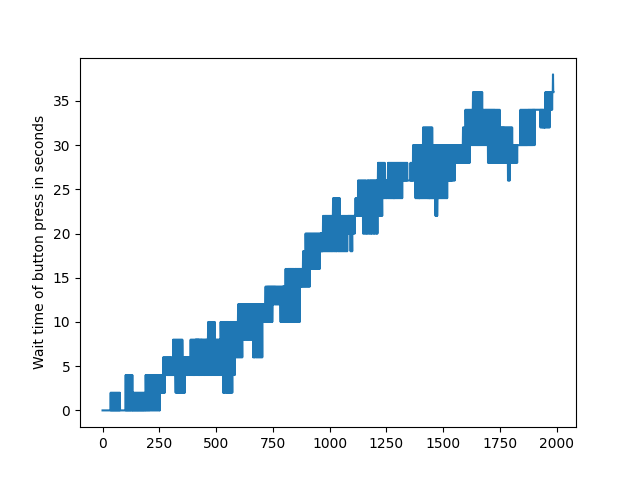
\includegraphics[scale=0.5]{Figure_1.png}
    {\footnotesize \textbf{Figure 1.} The processing time in seconds for each sen batch of pictures.
    Always rising graph. \par} And with eigth edge nodes the gateway is
    running without any waiting time which shows in Figure 2. 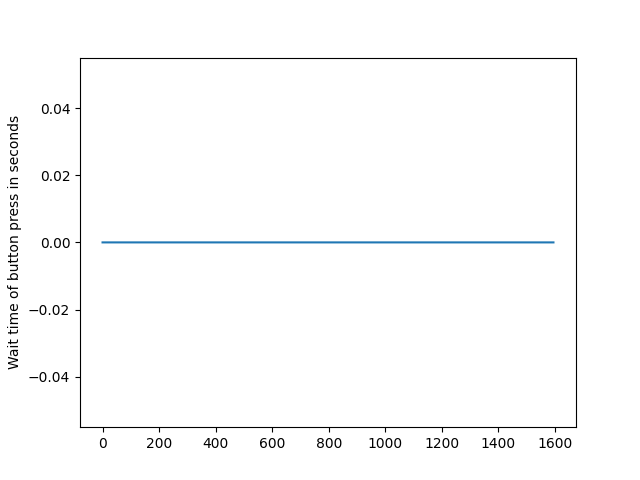
\includegraphics[scale=0.5]{Figure_2.png}
    {\footnotesize \textbf{Figure 2.} The processing time in seconds for each sen batch of pictures.
    Graph completely flat.\par} With nine nodes the gatway node is
    showing some times when it is not able to keep up but gets it down to a lower level also
    instead of the waiting times getting higher all the time which is contained in Figure 3.
    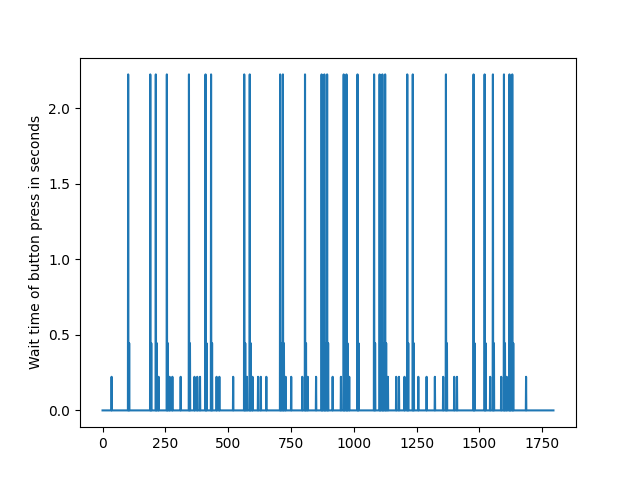
\includegraphics[scale=0.5]{Figure_3.png} {\footnotesize \textbf{Figure 3.} The processing time
    in seconds for each sen batch of pictures. Graph unstable but not rising.\par}
    
  \section{Discussion}
    When at ten devices the processing time will be so long that the data which the gate receives
    will just build up and the time it takes for each batch of pictures will we longer each time.
    With this simulation basing the processing power of a Raspberry PI 3 there exists at the time
    of writing this article the successor Raspberry PI for with more computing power which
    might be one solution to be able to handle more edge nodes. The other might be to have lower
    resolution camera but that might impact how good the recognition software can identify
    the threat it is looking for. With nine camera devices it is possible to cover  a lot of
    ground where there are many open spaces but within city centers with many buildings it
    might not be enough to cover even all ground in close proximity to the gateway node
    and more clusters of one gateway node with nine edge nodes might be needed which
    is more expensive.
    
  \section{Conclusion}
    To see how a Raspberry PI gateway node can handle incoming data in the form of
    pictures taken and sent over a wireless network and process it to find
    any threats or crimes committed to be able to alert rescue personnel or
    law enforcement automatically. We conducted simulations in python using
    the pysim[2] library and found out that with a Raspberry PI 3 B+ Model
    we are able to handle nine edge devices sending pictures at rate of five
    pictures in a batch every ten seconds.
    
  \section{References}
    {[1] S. S. Bhattacherjee, S. Kumar, P. Rajalakshmi. 2019 IEEE 5th World Forum on Internet
    of Things (WF-IoT). "Emotion Detection IoT enabled Edge-node for Citizen Security" 2019. pages=925-930.\par}
    {[2] simpy.readthedocs.io/en/latest, accessed on November 8th 2020.\par}
    {[3] Adrian Rosebrock, Raspberry Pi Face Recognition, June 25 2018. Accessed on November 8 2020. Available:
    https://www.pyimagesearch.com/2018/06/25/raspberry-pi-face-recognition/\par}
    {[4] A Norberg, A Nadjati, iot-simpy-sim, Noveber 2020. Acced on November 8 2020. Available:
    https://github.com/ackee/iot-simpy-sim\par}

  \onecolumn
  \section{Appendix - source code.}
  \begin{verbatim}
  """

Scenario:
  Simulation of several iot devices (sensors) needing to receive calculated data
  from their connected server.
  If the calculation is heavy the server needs to send a request to a supercomputer
  which will handle the computation.

"""
import random

import simpy

import matplotlib.pyplot as plt

# All times unless otherwise specified are in half a second

RANDOM_SEED = 42                 # Not so random but we want it reproducible
NUM_MACHINES = 1                 # Number of available machines in the cloud.
NUM_CORES = 4                    # Number of cpu cores on the raspberry pi.
NUM_DEVICES = 8                 # Number of edge devices
PROCESS_TIME = 8                 # Time it takes to calculate 
SEND_TO_CLOUD_TIME = 1           # Time it takes for a heavy calculation
SEND_INTERVAL = 20               # How often a edge device will send a bulk of five images.
SIM_TIME = 4000                  # Simulation time in seconds

time_data = []          # List of dictionaries to store the data of how long a request takes.

class Cloud(object):
    """
    A cloud with limited number of rented machines A.K.A The cloud.

    Gateway nodes can request one of the machines (1 default). When they get one
    the calculation can start. It takes processtime seconds.
    """
    def __init__(self, env, num_machines, processtime):
        self.env = env
        self.machine = simpy.PriorityResource(env, num_machines)
        self.processtime = processtime

    def calc(self, val):
        """
        The calculation processes. It takes a ``val`` processes and tries
        to calculate it.
        """
        yield self.env.timeout(self.processtime)

class Gateway(object):
    """
    Our gateway devices, hopefully only one is needed.
    """
    def __init__(self, env, num_servers, processtime, cloud):
        self.env = env
        self.server = simpy.PriorityResource(env, num_servers)
        self.processtime = processtime
        self.cloud = cloud
        self.reqsUntilSend = 10

    def proc(self, val):
        """
        Processing the data incoming from a IOT device.
        """

        #Every 10 requests we also send data to the cloud.
        if self.reqsUntilSend <= 0:
            self.reqsUntilSend = 10
            print("Gateway is sending data to the cloud!")
            yield self.env.timeout(random.randint(self.processtime-2, self.processtime+1))
            yield env.process(self.cloud.calc(val))
        else:
            # Every other when we don't send data to the cloud.
            self.reqsUntilSend = self.reqsUntilSend - 1
            yield self.env.timeout(self.processtime)


def device(env, name, gateway):
    """The device process (each device has a ``name``) sends a request for data
    from (``server``).

    It then starts the calculation process and waits for it to finish...

    """
    
    starttime = env.now
    with gateway.server.request() as request:
        yield request

        getsprocessed = env.now
        yield env.process(gateway.proc(name))

        getsanswered = env.now
        wt = getsprocessed - starttime
        pt = getsanswered - getsprocessed
        tt = getsanswered - starttime
        time_data.append({"waitTime": wt*2, "processTime": pt*2, "totalTime": tt*2})

def setup(env, num_devices, num_machines, num_cores, processtime, computetime, t_inter):
    """Create a cloud, a number of servers, a number of initial device requests and keep creating cars
    approx. every ``t_inter`` minutes."""
    # Create the Cloud object
    cloud = Cloud(env, num_machines, computetime)

    # Create the Gateway system
    gateway = Gateway(env, num_cores, processtime, cloud)

    i=0
    # Create more iot data requests while the simulation is running
    while True:
        yield env.timeout(t_inter/num_devices)
        i+=1
        env.process(device(env, 'IOT %d' % (i%num_devices), gateway))

# Setup and start the simulation
print('IOT Network simulation')

random.seed(RANDOM_SEED)  # This helps reproducing the results

# Create an environment and start the setup process
env = simpy.Environment()
env.process(setup(env, NUM_DEVICES, NUM_MACHINES, NUM_CORES, PROCESS_TIME, SEND_TO_CLOUD_TIME, SEND_INTERVAL))

# Execute!
env.run(until=SIM_TIME)


print([item["waitTime"] for item in time_data])

plt.plot([i["waitTime"] for i in time_data])
plt.ylabel("Wait time of button press in seconds")
plt.show()

  \end{verbatim}
\end{document}
